\documentclass[10pt,a4paper]{report}

\usepackage[utf8]{inputenc}
\usepackage[french]{babel}
\usepackage[T1]{fontenc}
\usepackage{amsmath}
\usepackage{amsfonts}
\usepackage{amssymb}
\usepackage{graphicx}
\usepackage{lmodern}
\usepackage[left=2cm,right=2cm,top=2cm,bottom=2cm]{geometry}

\usepackage{hyperref}
\usepackage{xspace}

\author{Alexia HOCINE}
\title{Stage M2 Physique, parcours SUBA\\Université de Claude Bernard Lyon 1}
\date{2021-2022}

% raccourci français
\newcommand{\cad}{c'est-à-dire\xspace}

% nom informatique
\newcommand{\ROOT}{\texttt{ROOT}\xspace}
\newcommand{\SLCIO}{\texttt{SLCIO}\xspace}
\newcommand{\processor}{\texttt{processor}\xspace}
\newcommand{\analysis}{\texttt{analysis}\xspace}
\newcommand{\nnhAnalysis}{\texttt{nnhAnalysis}\xspace}


\begin{document}

\maketitle

\chapter*{Préambule}

\paragraph{Email Gérald Grenier :}

\subparagraph{Un tutorial de \texttt{ilcsoft} :} 
\url{https://agenda.linearcollider.org/event/9272/}

\subparagraph{Initialisation \texttt{ilcsoft} :}
%source /cvmfs/ilc.desy.de/sw/x86_64_gcc82_centos7/v02-02-03/init_ilcsoft.sh

\subparagraph{La documentation et le packet \texttt{git} du format de données \texttt{LCIO} et de la librairie \texttt{Marlin}}
\begin{itemize}
	\item \url{https://github.com/iLCSoft/LCIO}
	\item \url{https://github.com/iLCSoft/Marlin}
\end{itemize}


\subparagraph{Pour la deuxième partie du stage :}
\begin{itemize}

	\item le software en développement : 
			\url{https://github.com/key4hep}
			
	\item et plus particulièrement l'adaptateur \texttt{ilcsoft} vers \texttt{key4hep} : 
			\url{https://github.com/key4hep/k4MarlinWrapper}
			
\end{itemize}  

\part{\texttt{ilcsoft}}

\chapter{Projet \nnhAnalysis}

\section{Programme \processor}

\subsection{Données}
Initialement, on m'a mis à disposition des fichiers \SLCIO rangés par processus dans 66 dossiers (Figure~\ref{listeProcessus}).

\begin{figure}[h!]
	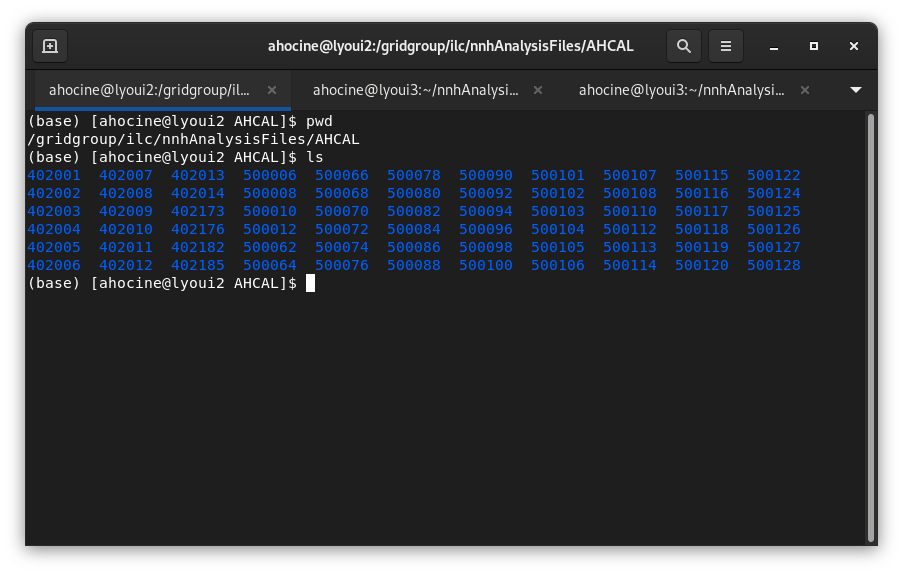
\includegraphics[width= \textwidth]{img/listeProcessus.png} 
	\caption{Les noms des dossiers qui correspondent aux numéros de processus}
	\label{listeProcessus}
	
\end{figure}

\paragraph{Numéro des processus ???}

%\paragraph{Résultats mis à disposition ???}

\subsection{Méthodes}

On cherche à convertir ces fichiers \SLCIO en arbre \ROOT par processus.

\subsection{Résultats}

%\paragraph{Des fichiers \ROOT :}
Chaque dossier de fichier de donnée \SLCIO produira un fichier \ROOT en sortie, \cad que l'on obtiendra un arbre \ROOT par processus.


\subsection{Interprétation}

\section{Programme \analysis}

\subsection{Données}

On récupère les fichiers \ROOT du programme \processor précédent. 

$ hadd $ qui va créer le fichier DATA.root

\subsection{Méthodes}

\subsubsection{\texttt{BDT}}

Entrainement

\subsubsection{L'analyse}



\subsection{Résultats}

\subsubsection{Vérification des résultats}
Comparaison entre les différents séries d'analyse, basée sur les même fichiers \ROOT, mais un autre entraînement de BDT.

\subsection{Interprétation}

\part{\texttt{fcc}}

\end{document}